\documentclass[11pt,a4paper]{article}
\usepackage[utf8]{inputenc}
\usepackage{amsmath}
\usepackage{amsfonts}
\usepackage{amssymb}
\usepackage{enumerate}
\usepackage{graphicx}
\usepackage{enumitem}



\title{Lab 02\\Arquitectura de Computadores \\ \Large{Sección 2}}
\author{Joaquín Ramírez}
\date{Mayo 04, 2020}
\begin{document}
\maketitle
\begin{enumerate}
\item Será implementado en el ejercicio 2.a
\item
\begin{enumerate}[label=(\alph*)]
\item Implementación de un 2-to-1 MUX de 16-bits.La implementación es igual que un MUX 2x1 de 1 bi. La complejidad no requirió separar los módulos en $small$ y $top$. Se probaron 10 tiempos, en los que cada un segundo $a$ disminuye en 1, mientras que $b$ aumenta en 1 cada dos segundos. Se observa que cuando el $select \  s$ está ``low", el valor de $y$ es el de $b$, y cuando está ``high", $y$ toma el valor de $a$. El diagrama en $GTKWave$ comprueba la tabla de verdad.
\begin{figure}[h!]
\centering
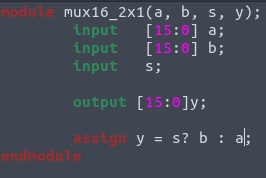
\includegraphics[scale=0.6]{16_2x1MUX_1.png} 
\end{figure}
\begin{figure}[h!]
\centering
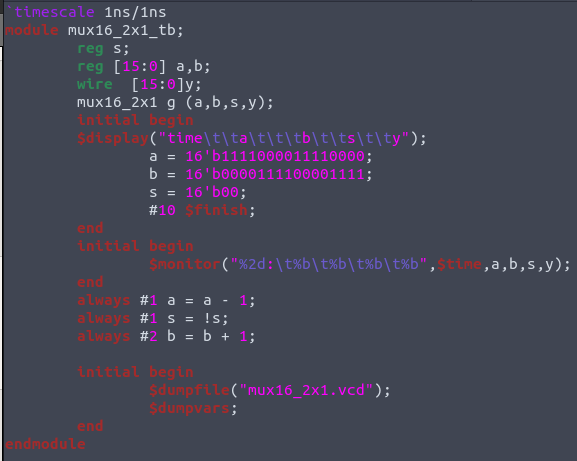
\includegraphics[scale=0.35]{16_2x1MUX_2.png} 
\end{figure}
\pagebreak
\begin{figure}[h!]
\centering
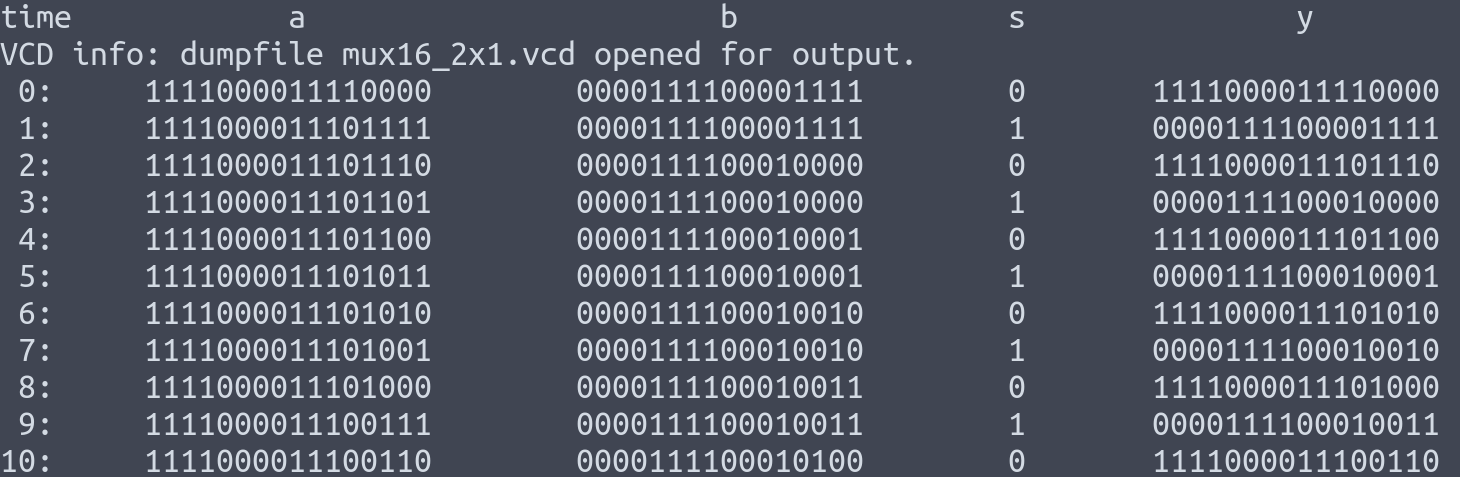
\includegraphics[scale=0.4]{16_2x1MUX_3.png} 
\end{figure}\\
\begin{figure}[h!]
\centering
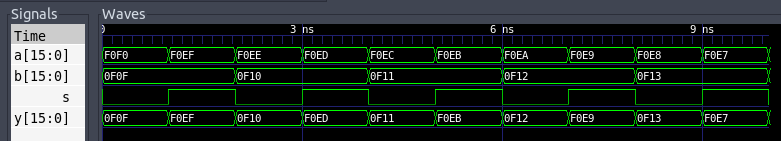
\includegraphics[scale=0.4]{16_2x1MUX_4.png} 
\end{figure}
\item Implementación de un 8-to-1 MUX de 16-bits. Se crearon por separado módulos de OR, AND y NOT gate (small), y se llamaron en el top. En el test bench se puede apreciar que para cada combinación entre selects, el output es un input único. La tabla de verdad coincide con la representación en   $GTKWave$.
\begin{figure}[h!]
\centering
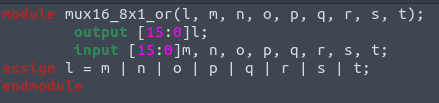
\includegraphics[scale=0.5]{16_8x1MUX_1.png} 
\end{figure}
\begin{figure}[h]
\centering
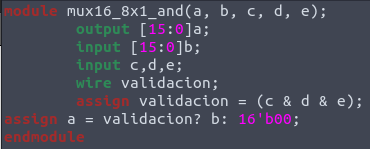
\includegraphics[scale=0.7]{16_8x1MUX_2.png} 
\end{figure}
\begin{figure}[h!]
\centering
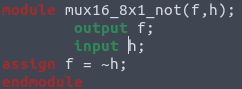
\includegraphics[scale=0.7]{16_8x1MUX_3.png} 
\end{figure}
\begin{figure}[h!]
\centering
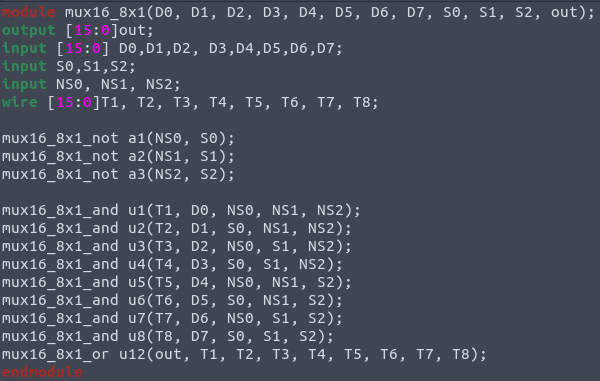
\includegraphics[scale=0.4]{16_8x1MUX_4.png} 
\end{figure}
\begin{figure}[h!]
\centering
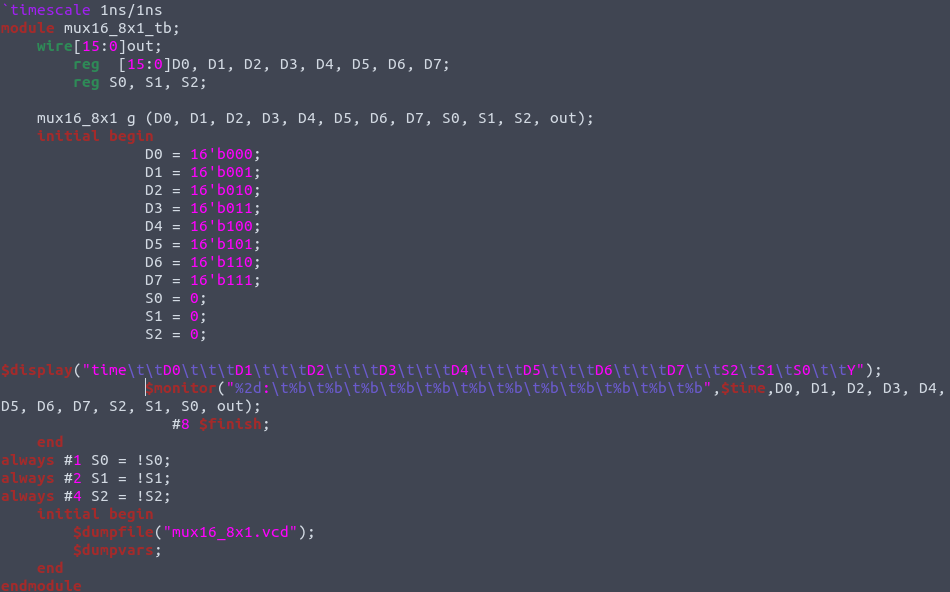
\includegraphics[scale=0.35]{16_8x1MUX_5.png} 
\end{figure}
\begin{figure}[h!]
\centering
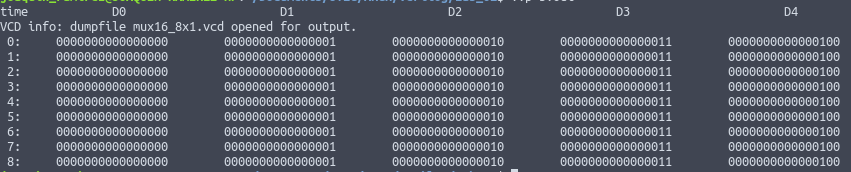
\includegraphics[scale=0.5]{16_8x1MUX_61.png} 
\end{figure}
\begin{figure}[h!]
\centering
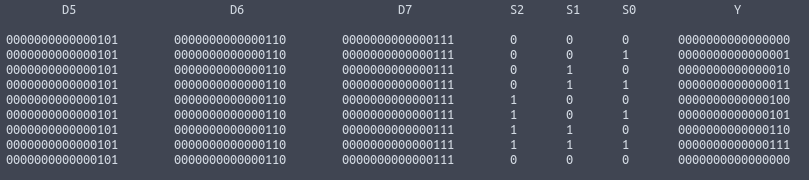
\includegraphics[scale=0.5]{16_8x1MUX_62.png} 
\end{figure}
\begin{figure}[h!]
\centering
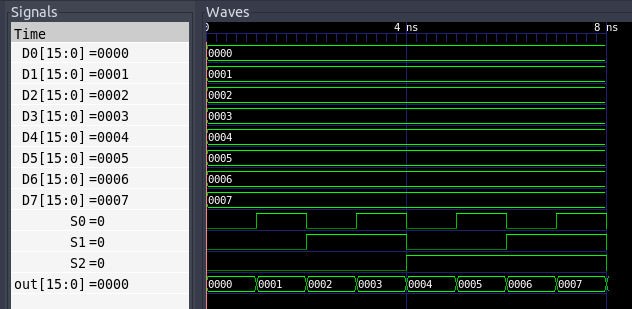
\includegraphics[scale=0.5]{16_8x1MUX_7.png} 
\end{figure}
\item Implementación de un 16-to-1 MUX de 16-bits. El mismo concepto previo, pero ahora hay que aumentar 8 inputs, por lo que un $select$ más es necesario,
\begin{figure}[h!]
\centering
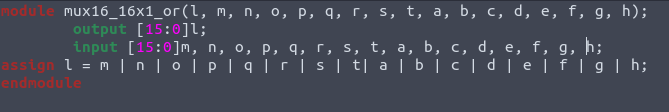
\includegraphics[scale=0.5]{16_16x1MUX_1.png} 
\end{figure}
\begin{figure}[h]
\centering
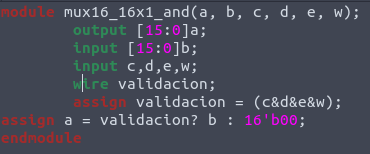
\includegraphics[scale=0.7]{16_16x1MUX_2.png} 
\end{figure}
\begin{figure}[h!]
\centering
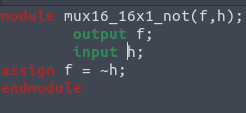
\includegraphics[scale=0.7]{16_16x1MUX_3.png} 
\end{figure}
\begin{figure}[h!]
\centering
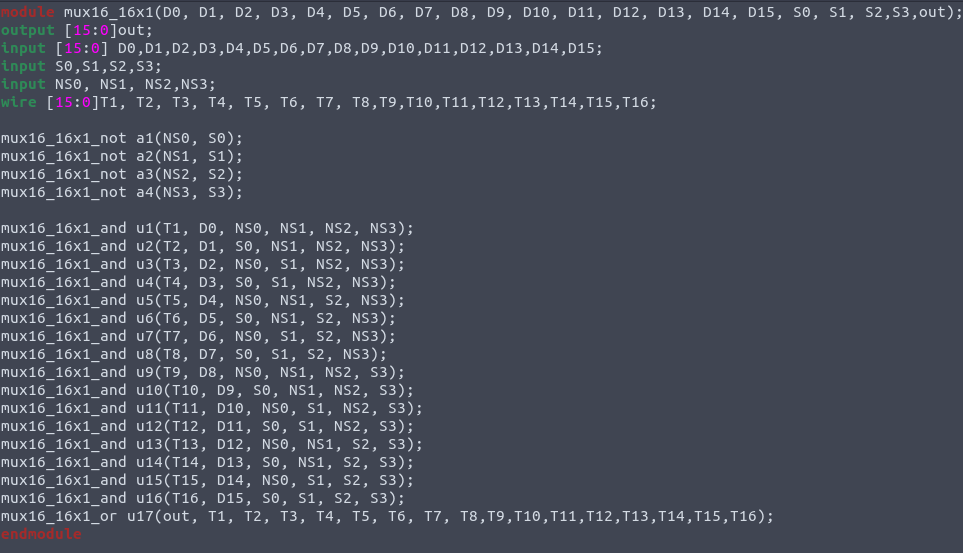
\includegraphics[scale=0.4]{16_16x1MUX_4.png} 
\end{figure}
\begin{figure}[h!]
\centering
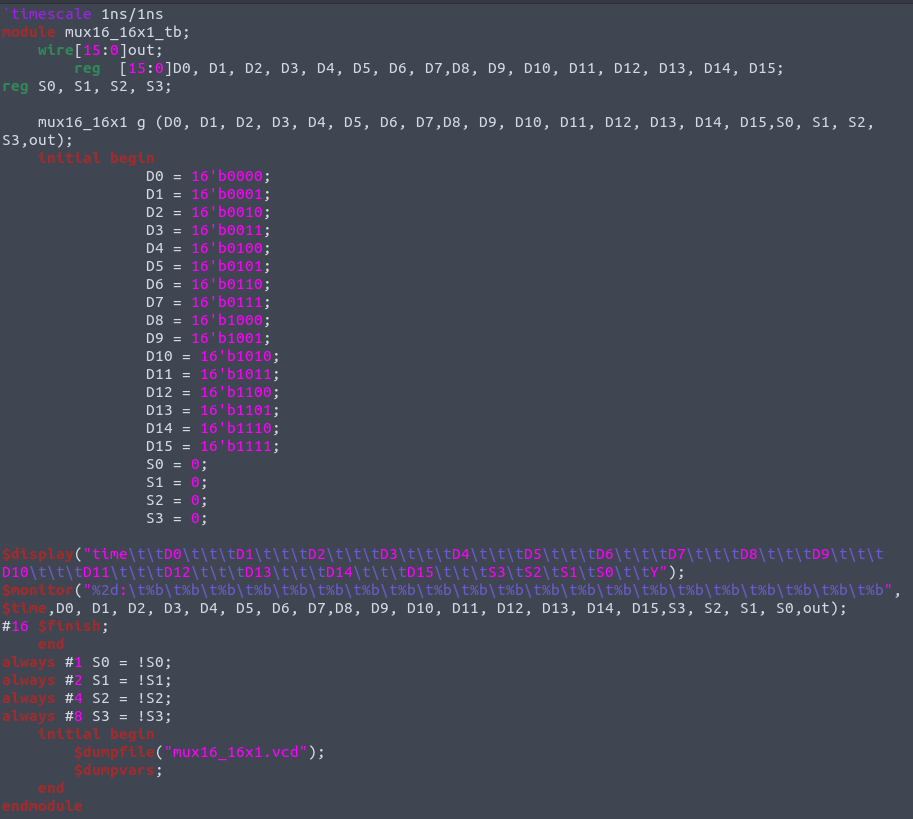
\includegraphics[scale=0.4]{16_16x1MUX_5.png} 
\end{figure}
\begin{figure}[h!]
\centering
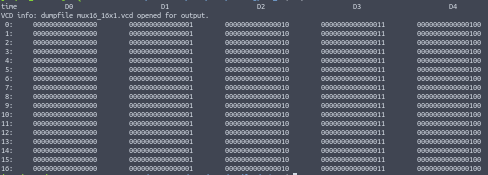
\includegraphics[scale=0.7]{16_16x1MUX_61.png} 
\end{figure}
\begin{figure}[h!]
\centering
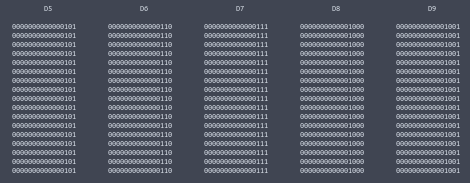
\includegraphics[scale=0.7]{16_16x1MUX_62.png} 
\end{figure}
\begin{figure}[h!]
\centering
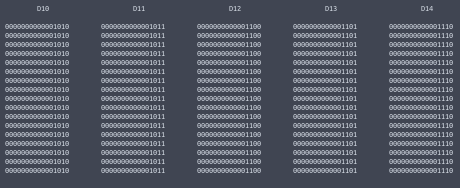
\includegraphics[scale=0.7]{16_16x1MUX_63.png} 
\end{figure}
\begin{figure}[h!]
\centering
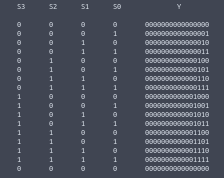
\includegraphics[scale=0.7]{16_16x1MUX_64.png} 
\end{figure}
\begin{figure}[h!]
\centering
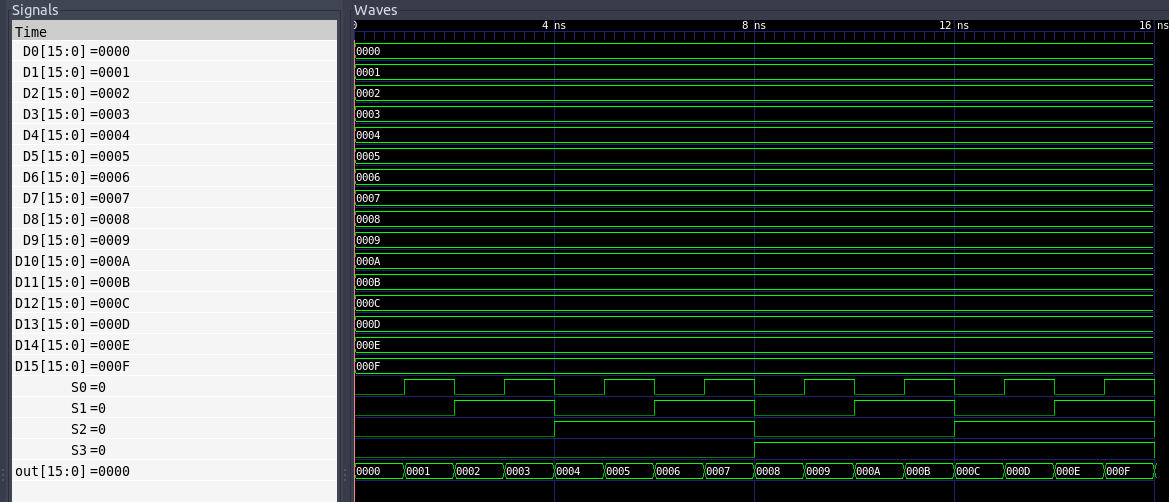
\includegraphics[scale=0.3]{16_16x1MUX_7.png} 
\end{figure}
\end{enumerate}
\item 
\item .
\item .
\item .


\end{enumerate}
\end{document}